\section{ИССЛЕДОВАНИЕ РАБОТЫ ОПЕРАТИВНОГО ЗАПОМИНАЮЩЕГО УСТРОЙСТВА}

К основным управляющим и информационным сигналам относятся:
\begin{itemize}
	
\item А0…Аn - адрес, или адресный код. Адресный код является номером элемента или ячейки памяти, в котором хранится бит, байт или слово информации. Число разрядов адресного кода «n» определяет емкость памяти ОЗУ. Например, 12-разрядный код A11A10A9...A0 позволяет обратиться к любой из 212 = 4048 ячеек памяти ОЗУ;

\item (CS) (Chip Select) или (СЕ) (Chip Enable) – сигналы выбора кристалла, или микросхемы, активизирующие работу микросхемы ОЗУ при
нулевом логическом уровне;

\item R/W (Read/Write) – сигнал, управляющий режимом работы памяти: при R/W = 0 производится запись, при R/W = 1 - чтение;

\item DI, DO (Data Input, Data Output) – входные и выходные m - разрядные данные ОЗУ, передаваемые по совмещенной или отдельным шинам. Число разрядов m определяется организацией ЗУ

\end{itemize}

\begin{figure}[H]
	\centering
	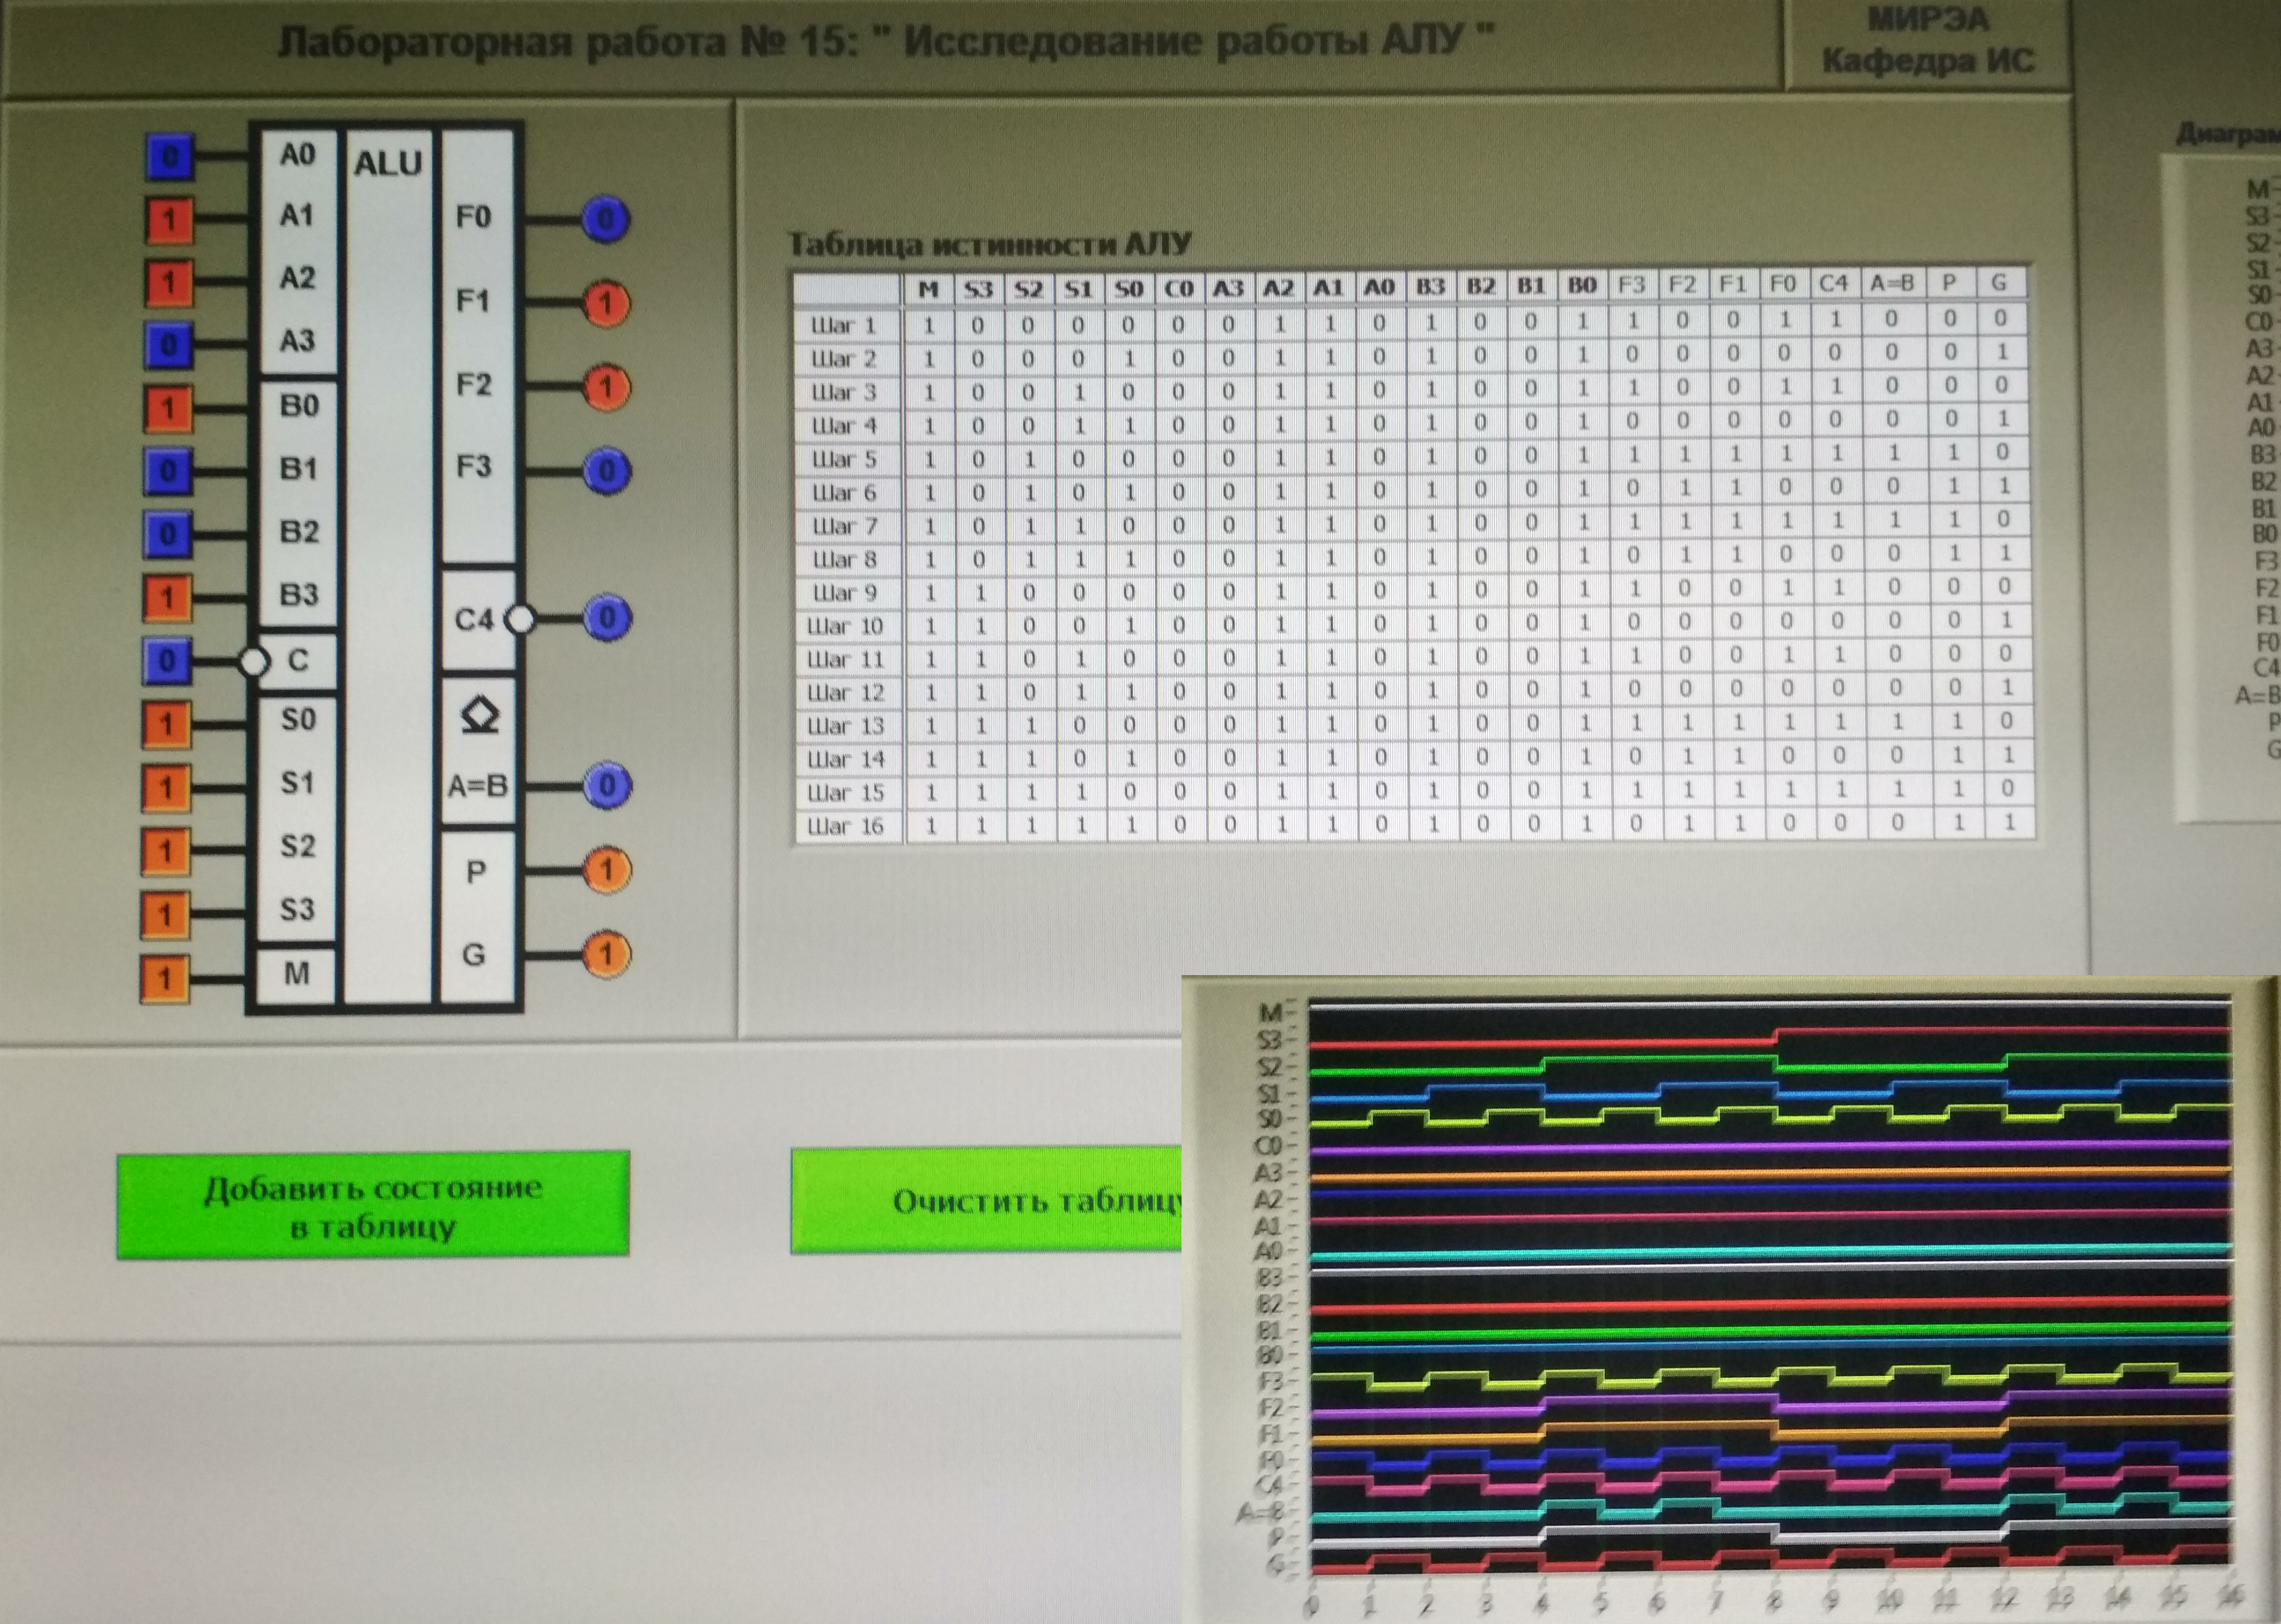
\includegraphics[width=0.95\linewidth]{imgs/16/1}
	\caption{РЕЖИМ ЗАПИСИ ДАННЫХ}
	\label{fig:16_1}
\end{figure}

\begin{figure}[H]
	\centering
	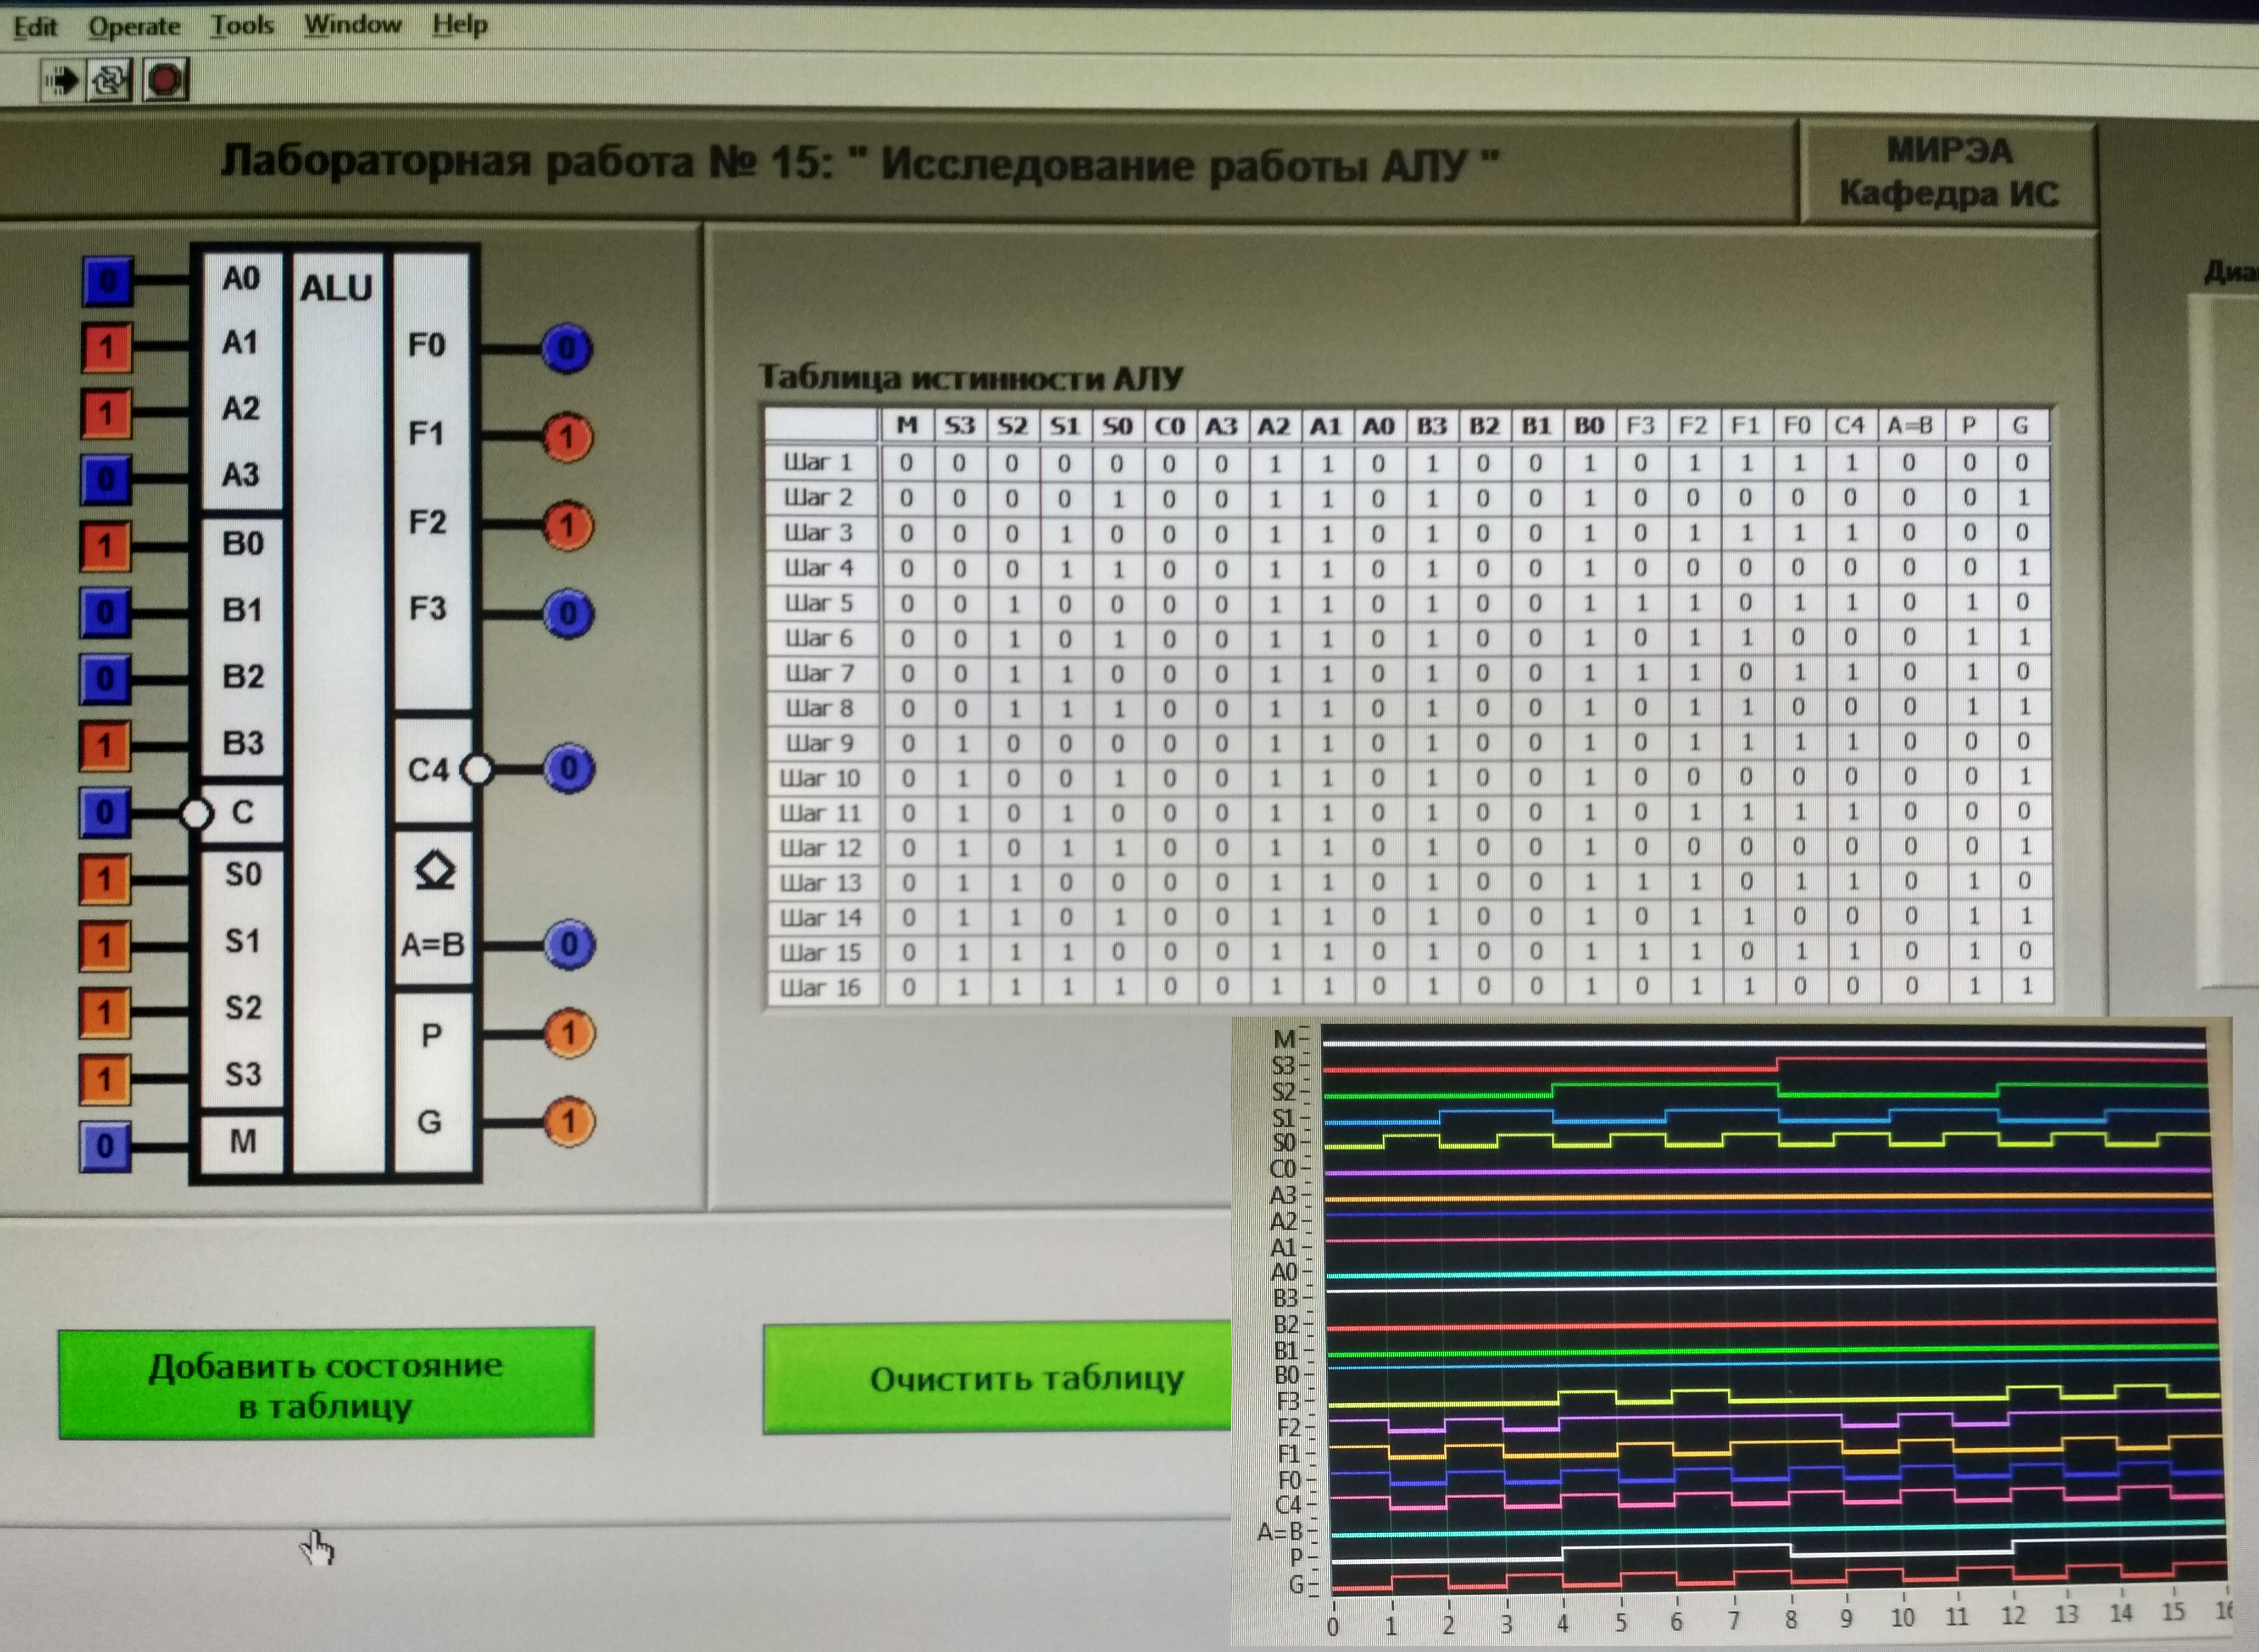
\includegraphics[width=0.95\linewidth]{imgs/16/2}
	\caption{РЕЖИМ ЧТЕНИЯ ДАННЫХ}
	\label{fig:16_2}
\end{figure}

Элемент SN74LS189 - Schottky Logic

Характеристики:

\begin{figure}[H]
	\centering
	\includegraphics[width=0.7\linewidth]{imgs/16/16_sh}
	\caption{Схема}
	\label{fig:16_sh}
\end{figure}

\begin{figure}[H]
	\centering
	\includegraphics[width=0.95\linewidth]{imgs/16/16_rec}
	\caption{Рекомендуемые параметры}
	\label{fig:16_rec}
\end{figure}

\begin{figure}[H]
	\centering
	\includegraphics[width=0.95\linewidth]{imgs/16/16_ch}
	\caption{Электрические характеристики}
	\label{fig:16_ch}
\end{figure}

\begin{figure}[H]
	\centering
	\includegraphics[width=0.95\linewidth]{imgs/16/16_switch}
	\caption{Коммутационные характеристики}
	\label{fig:16_switch}
\end{figure}
